% Architecture, Usage and Evaluation of the tool paper as a standalone document, to send for review.
% Source: paper/0{2,3,4} *.md. Compile from paper/latex: BIBINPUTS=..: latexmk -pdf draft_standalone.tex
\documentclass[11pt,a4paper]{article}
\usepackage[margin=2.2cm]{geometry}
\usepackage[T1]{fontenc}
\usepackage{lmodern}
\usepackage{graphicx}
\usepackage{booktabs}
\usepackage{amsmath}
\usepackage{caption}
\usepackage[section]{placeins}  % keeps each figure in its own section
\usepackage{listings}
\usepackage[hidelinks]{hyperref}
\lstset{basicstyle=\ttfamily\footnotesize, columns=fullflexible, keepspaces=true, frame=single,
  framesep=4pt, xleftmargin=6pt, xrightmargin=6pt, breaklines=true, showstringspaces=false}
\captionsetup{font=small}

\newcommand{\code}[1]{\texttt{#1}}
\emergencystretch=3em  % long file paths in \code would otherwise run into the margin

\title{Concrete QUANTAS: Architecture, Usage and Evaluation}
\author{}
\date{Draft, \today}

\begin{document}
\maketitle

\section{Architecture}

Concrete QUANTAS runs QUANTAS algorithms on real operating system processes. Its generic runtime
knows nothing about how messages travel: everything specific to a communication technology sits
behind a small backend interface. We have implemented two backends, BoostMq and ZeroMQ.

\subsection{From Abstract to Concrete}

In Abstract QUANTAS~\cite{quantas}, a single process simulates every peer in rounds, and channels
model message delay. An algorithm is a subclass of \code{Peer} that implements
\code{performComputation()} and sends messages through a \code{NetworkInterface}.

Concrete QUANTAS keeps this programming model, and an algorithm written for Abstract QUANTAS runs on
it unchanged. The runtime needs only two answers that a generic \code{Peer} cannot give: whether a
peer has finished, so that the leader can stop a test once every correct peer has, and which values
to report. A small \emph{algorithm adapter}, kept in its own file, provides them by reading the
algorithm's public state, much as an Abstract algorithm's results file reads it at the end of a
simulation.

The execution model is what changes. Each peer is its own process, and a separate leader process
coordinates them. A launcher starts these processes from one JSON input file. The leader validates
the input, plans the topology and writes the final report. Each peer runs a loop: receive pending
messages, perform its computation, report delivery the first time it happens, and repeat every
10\,ms until it is told to stop or its time window ends. Time is therefore real rather than
simulated: delays come from the system, and an experiment is bounded by a time window instead of a
number of rounds.

\subsection{One architecture for both}

Figure~\ref{fig:uml} extends the architecture of the original QUANTAS paper~\cite{quantas}. The
original components keep their names, with the class that implements each one in parentheses. The
user still provides the Configuration, the Concrete Node (the algorithm) and the User-Defined
Message, and the Abstract Node, the Node Network Interface and the Packet are shared by both
versions. Abstract QUANTAS keeps its Simulation and Network, which run every node in one process, in
rounds. Its Node Network Interface becomes one implementation among several: the original one moves
messages through simulated channels with delays.

Concrete QUANTAS adds the parts shown in orange. A Leader Process reads the same Configuration, and
each node runs in its own Peer Process. A Backend builds a Coordinator for control messages and a
Node Network Interface for data, with one implementation each for BoostMq and ZeroMQ. The user may
add an Algorithm Adapter next to the Concrete Node.

\begin{figure}[!htbp]
  \centering
  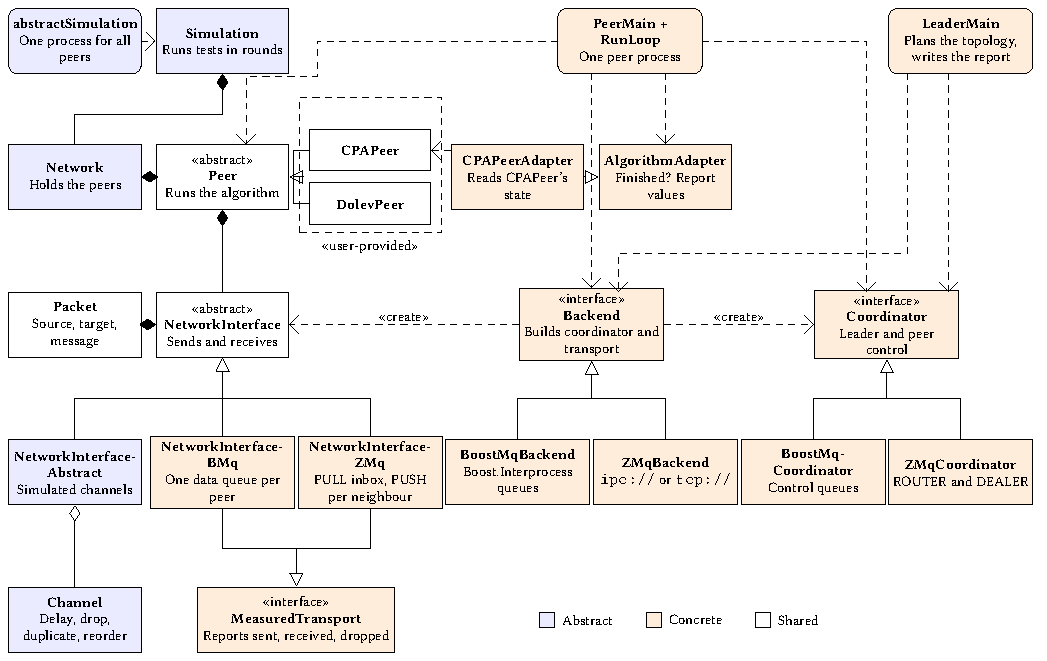
\includegraphics[width=\textwidth,height=0.62\textheight,keepaspectratio]{../figures/quantas-uml.pdf}
  \caption{The QUANTAS architecture of~\cite{quantas}, extended with Concrete QUANTAS. Class names
    are in parentheses. Blue components exist only in Abstract QUANTAS, orange ones are added by
    Concrete QUANTAS, and white ones are shared. Filled diamonds show composition, the hollow diamond
    aggregation, hollow triangles inheritance (dashed: implements an interface), solid arrows use,
    and dashed arrows dependencies; both processes use the Backend and the Coordinator through the
    shared dashed line. Boxes with rounded corners are processes.}
  \label{fig:uml}
\end{figure}

\subsection{Backend interface}

The runtime talks to a backend through three interfaces:
\begin{itemize}
  \item \code{Backend} reads the backend's settings, checks before a run that the experiment can
    execute, and creates the two objects below. \code{BackendFactory} selects it from the
    \code{backend} field of the input.
  \item \code{Coordinator} is the control plane: the messages between the leader and the peers that
    run each test.
  \item \code{NetworkInterface} is the data plane: the transport that carries the algorithm's
    messages. Each backend's transport also implements \code{MeasuredTransport}, which reports the
    messages sent, received and dropped.
\end{itemize}
Because \code{Backend} creates a matching coordinator and transport, the leader, the peer loop and
the algorithms depend only on these interfaces. Adding a backend means implementing them and adding
one line to the factory.

\subsection{Control protocol}

Every test follows the same protocol on both backends:
\begin{enumerate}
  \item Each peer opens its channels and sends READY to the leader.
  \item The leader waits for every peer, then sends each one its assignment: its identifier and its
    neighbours.
  \item Each peer creates its transport and algorithm object, then waits. The leader sends START to
    all peers.
  \item Peers run the algorithm. A correct peer sends DELIVERED the first time it delivers.
  \item Once all correct peers have delivered, the leader sends STOP. Without STOP, a peer stops
    when its time window ends.
  \item Each peer writes its metrics to a file and sends DONE, or FAILED if an error occurred.
  \item The leader reads the metrics files and adds the test to its report.
\end{enumerate}
The leader bounds its waits with timeouts. A timeout, a FAILED message or an invalid metrics file
marks the test as failed rather than letting the run hang. A data send that times out does the
same, so a full queue fails the test instead of silently dropping the message.

\subsection{Backends}

\textbf{BoostMq} uses Boost.Interprocess message queues in shared memory~\cite{boost-interprocess},
so all processes must run on one machine. The leader creates two control queues,
\code{mq\_barrier} for READY and \code{mq\_done} for DELIVERED, DONE and FAILED. Each peer creates a
control queue for its assignment, START and STOP, and a data queue that serves as its inbox. A
sender opens the destination's data queue and waits at most 10\,ms by default when it is full.

\textbf{ZeroMQ} uses sockets~\cite{zeromq-patterns}, with the same protocol but a different
structure. For control, the leader binds one ROUTER socket and each peer connects one DEALER socket,
so the leader can reach any peer by its routing identifier. For data, each peer binds one PULL
socket as its inbox and connects one PUSH socket to each neighbour. Sockets that stay in a known
place bind, and the others connect, so ZeroMQ's automatic reconnection makes the start order of
peers irrelevant. ZeroMQ also needs one extra control message, RELEASE, which tells a peer that the
test is over and that it may start the next one. BoostMq signals this by having the leader remove
the peer's control queue.

ZeroMQ runs over \code{ipc://} on one machine and over \code{tcp://} on a cluster. The choice
depends only on the input: setting \code{leaderHost} and \code{peerHosts} selects \code{tcp://}.
Peer $i$ then runs on \code{peerHosts[i \% size]} and listens on port \code{basePort + 1 + i}, so
any peer can compute the address of any neighbour. Neither the algorithms nor the socket types
change. On a cluster, the nodes need a shared folder, because the leader reads the metrics files
that the peers write.

\section{Using Concrete QUANTAS}

This section shows how to prepare an algorithm, write an input file, run an experiment on one
machine, and move it to a cluster.

\subsection{Preparing an algorithm}

An algorithm for Concrete QUANTAS is written exactly as for Abstract QUANTAS: a \code{Peer} subclass
with \code{performComputation()}, using the same messaging calls, such as \code{broadcast} and
\code{unicastTo}. Its files are not changed. The MT-CPA code we run on all backends is the original
Abstract implementation, byte for byte.

The Concrete runtime needs two answers that the algorithm's own code does not give: whether a peer
has finished, so the leader can stop a test once every correct peer has, and which values to put in
the report. An \emph{algorithm adapter} provides them in a separate file,
\code{Concrete/Adapters/<Name>Adapter.cpp}, by reading the algorithm's public state. For MT-CPA:
\begin{lstlisting}[language=C++]
static const bool registered = registerAlgorithmAdapter<CPAPeer>(
    [](const CPAPeer& peer) { return peer.delivered; },    // finished?
    [](const CPAPeer& peer) {                               // values for the report
        return nlohmann::json{{"delivered", peer.delivered},
                              {"delivered_value", peer.mDelivered},
                              {"messages_sent", peer.msgsSent}, ...};
    });
\end{lstlisting}
The build links the adapter of every algorithm named in the input. An algorithm without an adapter
still runs, but the leader cannot stop a test early, and the report has no algorithm values.

\subsection{Writing an input file}

Concrete QUANTAS uses the same JSON format as Abstract QUANTAS, with a few additional settings:
\begin{lstlisting}
{
  "algorithms": ["CPAPeer/CPAPeer.cpp"],
  "experiments": [{
    "backend": "zeroMq",
    "windowMs": 2000,
    "doneTimeoutMs": 120000,
    "zeroMq": {"dataQueueCapacity": 20000},
    "logFile": "example.json",
    "tests": 2,
    "rounds": 1000,
    "threadCount": 1,
    "distribution": {"type": "GEOMETRIC", "maxDelay": 20},
    "topology": {
      "type": "complete",
      "initialPeers": 6,
      "initialPeerType": "CPAPeer"
    },
    "parameters": {"sender": 0, "ts": 1, "tl": 1, "byzantines": [3]}
  }]
}
\end{lstlisting}
The Concrete settings are:
\begin{itemize}
  \item \code{backend} selects \code{boostMq} or \code{zeroMq}. The default is \code{zeroMq}.
  \item \code{windowMs} is the longest time a peer runs in one test. The default is 2,000\,ms.
  \item \code{doneTimeoutMs} is how long the leader waits for the peers to report. The default is
    30,000\,ms.
  \item A block named after the backend holds its own settings, such as \code{dataQueueCapacity},
    the number of messages a peer's inbox can hold.
\end{itemize}
Both \code{windowMs} and \code{doneTimeoutMs} also accept \code{"infinite"}, which removes the limit.
We use this for the correctness check in the Evaluation section.

The other fields keep their Abstract meaning, with two differences. Concrete QUANTAS still requires
\code{rounds} but stops on \code{windowMs} instead. It also does not read \code{distribution},
because delays come from the real system. \code{tests} sets how many times each experiment repeats,
with the same network and the same parameters.

\subsection{Backend settings}

Each backend has its own settings block. Defaults suit small experiments, but heavier ones may need
larger queues. For BoostMq, all the settings are:
\begin{lstlisting}
"backend": "boostMq",
"boostMq": {
  "dataQueueCapacity": 20000,
  "maxMessageSizeBytes": 4096,
  "dataSendTimeoutMs": 10,
  "controlSendTimeoutMs": 5000,
  "readyTimeoutMs": 30000
}
\end{lstlisting}

\begin{table}[!htbp]
  \centering
  \small
  \begin{tabular}{@{}lrp{3.2cm}p{3.4cm}p{3.1cm}@{}}
    \toprule
    Setting & Default & Meaning & If too low & If too high \\
    \midrule
    \code{dataQueueCapacity} & 1,000 & Messages a peer's inbox can hold & The inbox fills, sends time
      out and the test fails & More shared memory \\
    \code{maxMessageSizeBytes} & 4,096 & Largest message allowed & Larger messages are rejected &
      More shared memory \\
    \code{dataSendTimeoutMs} & 10 & How long a send waits on a full inbox & A slow peer causes
      failures sooner & A peer can stall longer before failing \\
    \code{controlSendTimeoutMs} & 5,000 & How long the leader waits to send a control message &
      False failures under load & Failures take longer to appear \\
    \code{readyTimeoutMs} & 30,000 & How long the leader waits for every peer's READY & Slow
      start-up fails the test & A dead peer takes longer to detect \\
    \bottomrule
  \end{tabular}
  \caption{BoostMq settings.}
  \label{tab:boostmq}
\end{table}

\paragraph{Memory.} BoostMq's data queues need shared memory of about
\[ \text{peers} \times \texttt{dataQueueCapacity} \times \texttt{maxMessageSizeBytes}. \]
With 100 peers and the values above, this is about 7.8\,GB in \code{/dev/shm}, so check the space
available before raising these values.

\paragraph{Effect on results.} A full queue makes the test fail instead of silently dropping the
message, so a capacity that is too low appears as a failed experiment, not as lower liveness or
safety. Concrete QUANTAS has no simulated delays: these timeouts only decide when to give up, so they
should not change the outcome of a healthy run.

\paragraph{ZeroMQ.} ZeroMQ has \code{dataQueueCapacity}, \code{dataSendTimeoutMs} and
\code{readyTimeoutMs}, with the same defaults, but no \code{maxMessageSizeBytes} or
\code{controlSendTimeoutMs}. Its capacity also means something different. ZeroMQ applies the limit
per connection, on both ends, so a send to a stalled peer times out after about twice the capacity.
Its memory also grows as messages queue, instead of being reserved up front.

\subsection{Running on one machine}

The build compiles only the algorithms that the input names, so rebuild when switching to a
different algorithm:
\begin{lstlisting}
make mq_release INPUTFILE=example.json
bash quantas/Common/Concrete/Backends/BoostMq/Entrypoints/runBoostMq.sh \
    example.json ./quantas_mq_leader.exe ./quantas_mq_peer.exe /dev/shm
\end{lstlisting}
The same launcher runs both backends, and the input selects which one is used.
\code{make mq INPUTFILE=example.json} performs both steps in one command and removes any leftover
queues.

The leader writes its report to \code{Results/01EXP\_<name>/leader\_report.json}. For each test,
\code{algoReliability} holds the algorithm's metrics: liveness (\code{avg\_termination}), safety
(\code{avg\_safety}), delivery time and messages sent.

\subsection{Running on a cluster}

To run ZeroMQ across machines, add the machines' addresses to the input:
\begin{lstlisting}
"zeroMq": {
  "dataQueueCapacity": 20000,
  "leaderHost": "node1",
  "peerHosts": ["node2", "node3"],
  "basePort": 15555
}
\end{lstlisting}
Peer $i$ runs on \code{peerHosts[i \% size]}. Each machine then starts its processes from a folder
that all machines share, with one process per peer:
\begin{lstlisting}
# On the leader's machine
./quantas_mq_leader.exe --experiment 0 input.json

# On each peer's machine
./quantas_mq_peer.exe --experiment 0 input.json <peer_id>
\end{lstlisting}
The algorithm and the rest of the input stay the same. For the LIP6 cluster,
\code{experiments/\allowbreak cluster/\allowbreak run\_cluster.py} automates these steps: it reads the machines from the OAR
job, writes these settings, starts the processes and collects the results.

\section{Evaluation}
We evaluate Concrete QUANTAS with two questions. Does an algorithm behave the same on the Abstract
simulator and on real processes? And does the ZeroMQ backend hold up when the peers are spread
across machines? We answer both with the same experiments, run 10 times, on one cluster node and on
11 cluster nodes.

\subsection{Setup}

We use the MT-CPA algorithm and the experimental setup of Multi-Threshold Reliable
Communication~\cite{opodis-mtrc}.

\paragraph{Workload.} Each experiment has $n = 50$ peers, with peer 0 as the sender. We use the
$k = 3$ setting of that paper, with thresholds $(t_s, t_l) = (1, 1)$. The safety threshold $t_s$ is
the number of Byzantine peers up to which no correct peer delivers a value other than the sender's.
The liveness threshold $t_l$ is the number up to which every correct peer eventually delivers, on a
network with the required $k$-level ordering. MT-CPA counts these Byzantine peers per neighbourhood
rather than in the whole network. A peer that is not a neighbour of the sender delivers a value once
$t_s + 1$ neighbours have reported it. The paper sets $t_s + t_l = k - 1$ with both thresholds at
least 1, so $(1, 1)$ is the only pair at $k = 3$. There are three network families (edge remover,
Erd\H{o}s--R\'enyi and random regular), each with 10 \code{both} networks and 10 \code{dolev}
networks. A \code{dolev} network is $k$-connected. A \code{both} network also has a $k$-level
ordering, the condition MT-CPA relies on. We generate the networks at $n = 50$ with the method of
the paper's generators. The number of Byzantine peers $f$ runs from 1 to 5, which gives 300
experiments. All backends receive the same inputs: the networks and the Byzantine peers are
identical in every experiment.

\paragraph{Runs.} One run executes all 300 experiments once. We perform 10 runs on each backend and
deployment. Before the first run the nodes stay idle for 30 minutes, and between two runs for
10 minutes, so that no load from one run carries into the next. The runs share the networks and the
Byzantine peers and differ only in message timing. On Abstract, each run draws new message delays,
from a random seed based on the clock. On BoostMq and ZeroMQ, timing comes from real process
scheduling and transport. A single run is not enough: in an earlier test of one experiment with
$n = 100$, $k = 7$, $(1, 5)$ and $f = 5$, safety had a standard deviation of 10 to 15 points over
6 runs on every backend.

\paragraph{Byzantine behaviour.} Byzantine peers are chosen at random and fixed for each experiment.
They send a forged value in the first round and never forward messages.

\paragraph{Metrics.} \emph{Liveness} is the percentage of correct peers that deliver. \emph{Safety}
is computed as agreement: the percentage of delivering correct peers that hold the most common
value, which is not necessarily the sender's value. \emph{Delivery} is the average delivery time of
a peer. \emph{Messages} is the average number of messages sent per correct peer. Within a run, each
point in the figures is the mean over the 10 networks of one family and network type. Each point
therefore has 10 values, one per run. We report their mean and a 95\% confidence interval,
mean $\pm\, t_{0.975,9} \cdot s / \sqrt{10}$ with $t_{0.975,9} = 2.26$ and $s$ the standard
deviation over the runs.

\paragraph{Backends.} Abstract is a single process that simulates 1,000 rounds with geometric
message delays. BoostMq and ZeroMQ run each peer as an operating system process, with a time window
of 2\,s per run and a data queue capacity of 20,000 messages. The window plays the role of
Abstract's 1,000 rounds: it bounds a run in which some correct peers may never deliver. It is an
upper limit, not a fixed duration. The leader stops a run as soon as all correct peers have
delivered, so only runs in which some peer cannot deliver use the full 2\,s. Abstract reports
delivery in rounds and Concrete in milliseconds, so the two cannot be compared directly.

\paragraph{Deployments.} All experiments run on nodes of the LIP6 \code{small} cluster, one job at a
time.
\begin{itemize}
  \item \emph{One node:} Abstract, BoostMq and ZeroMQ over \code{ipc://} run on the same node, one
    after another and never in parallel. The leader and the 50 peers are processes on that node.
  \item \emph{11 nodes:} ZeroMQ over \code{tcp://}. The leader runs on one node and the 50 peers on
    the 10 others, 5 per node: peer $i$ runs on node $i \bmod 10$. Only the addresses in the input
    change; the inputs and settings are those of the one-node run.
\end{itemize}

\paragraph{Machine.} Each \code{small} node has an Intel Xeon E5645 processor at 2.40\,GHz with
24 logical CPUs and 62\,GB of RAM. It runs Debian, and we compile with g++ 14.2.0. The two jobs ran
one after the other: the one-node job first, then the 11-node job, each on its own nodes.

\subsection{Correctness}

We first check that the Concrete backends meet the guarantees of MT-CPA when its conditions hold.
We run every experiment within bounds, with $f \le \min(t_s, t_l)$, on \code{both} networks and with
no time limit, for $k = 3$, 5 and 7. In this setting every run must reach 100\% liveness and 100\%
safety.

Both backends pass: BoostMq and ZeroMQ each complete 420 of 420 experiments at 100\% liveness and
100\% safety, with no failures. This check ran once per experiment on a laptop (Intel Core Ultra 5
228V, 8 cores, 30\,GB of RAM).

The 10 runs on the cluster confirm it at $n = 50$. With $f = 1$, MT-CPA is within bounds for
$(1, 1)$, and on every \code{both} network, in every run, all four backends and deployments reach
100\% liveness and 100\% safety.

\subsection{Abstract vs Concrete on one node}

Every one of the 9,000 experiments (300 per run, 10 runs, 3 backends) completed without a failure.
Figure~\ref{fig:one-node} shows the results.

\begin{figure}[!htbp]
  \centering
  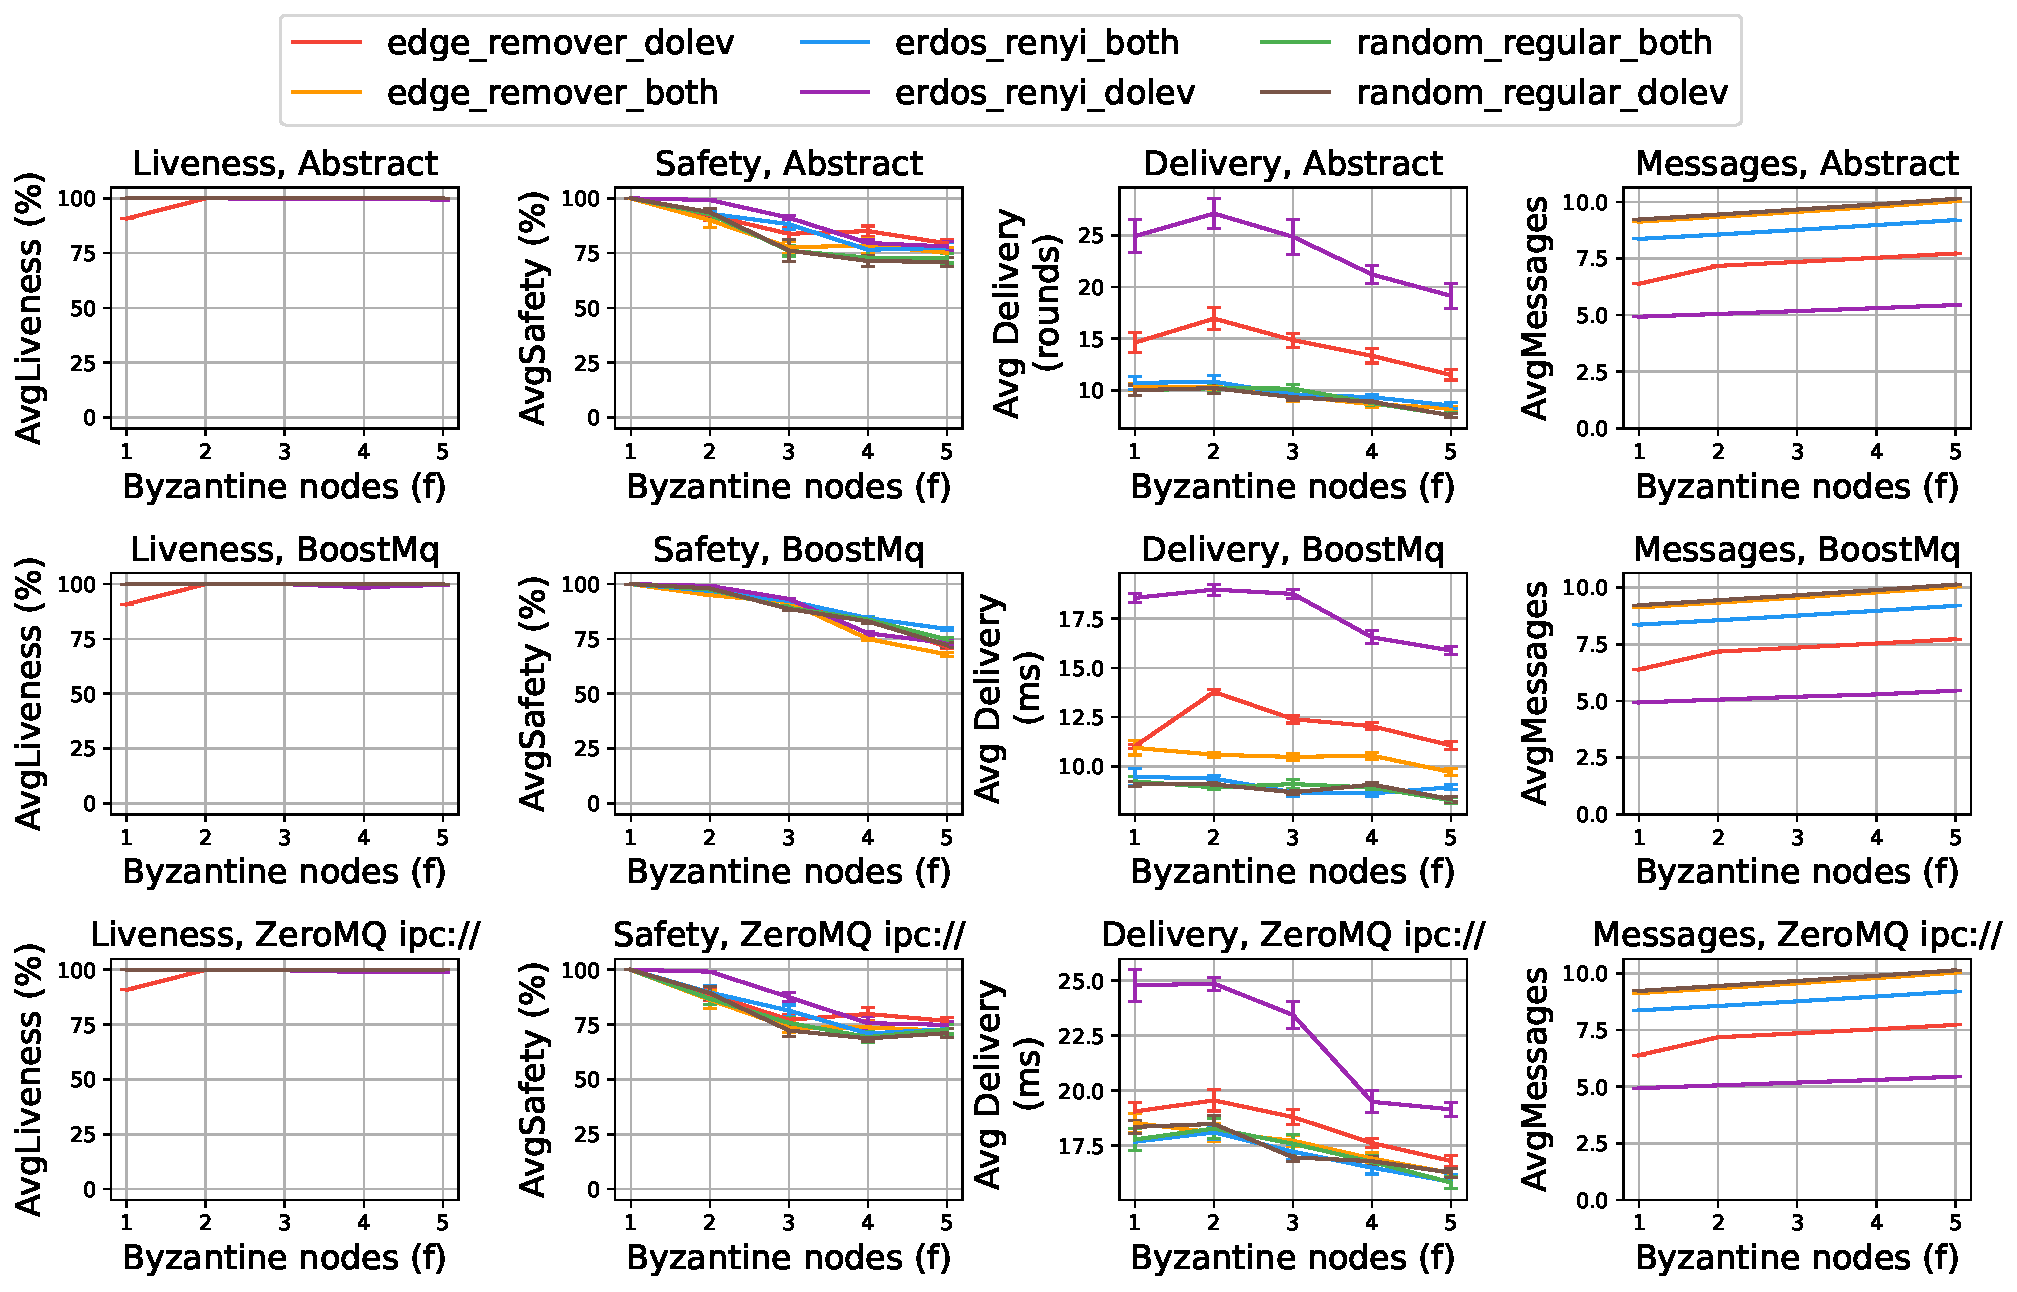
\includegraphics[width=\textwidth]{../figures/n50_one_node.pdf}
  \caption{MT-CPA with $n = 50$, $k = 3$ and $(t_s, t_l) = (1, 1)$ on one cluster node, for
    Abstract, BoostMq and ZeroMQ over \code{ipc://}. Each point is the mean over 10 runs of the mean
    over the 10 networks of one family and network type; error bars are 95\% confidence intervals
    over the runs. Delivery is in rounds for Abstract and in milliseconds for BoostMq and ZeroMQ.}
  \label{fig:one-node}
\end{figure}

\paragraph{Liveness} is the same on the three backends. The mean over all experiments is 99.7\% on
Abstract and 99.6\% on BoostMq and ZeroMQ. Liveness falls below 100\% only on \code{dolev} networks,
which lack the $k$-level ordering MT-CPA needs; on \code{both} networks it is 100\% at every $f$.

\paragraph{Messages} are the same as well. A correct peer sends 8.35 messages on average on every
backend. Per experiment, the mean over runs differs from Abstract by 0.02\% on average and by at
most 3.1\% (BoostMq) and 3.9\% (ZeroMQ).

\paragraph{Safety} is 100\% at $f = 1$ on all three backends and decreases as $f$ grows past
$t_s = 1$, to between 73\% and 76\% at $f = 5$. Between these ends, the backends differ by more than
the confidence intervals. Averaged over all networks, safety at $f = 3$ is 82.2\% on Abstract,
91.2\% on BoostMq and 78.0\% on ZeroMQ.

\paragraph{Delivery} cannot be compared in value between Abstract and Concrete, but its shape can.
On every backend, the \code{dolev} Erd\H{o}s--R\'enyi networks are the slowest, and delivery becomes
faster from $f = 2$ to $f = 5$. Averaged over all networks, a peer delivers after 10.4 to 14.3
rounds on Abstract, 10.4 to 11.8\,ms on BoostMq and 16.7 to 19.6\,ms on ZeroMQ, depending on $f$.

\subsection{ZeroMQ across 11 nodes}

ZeroMQ over \code{tcp://} also completed all 3,000 experiments without a failure, with the leader on
one node and 5 peers on each of the 10 others. Figure~\ref{fig:tcp} shows the results, on the same
axes as Figure~\ref{fig:one-node}.

\begin{figure}[!htbp]
  \centering
  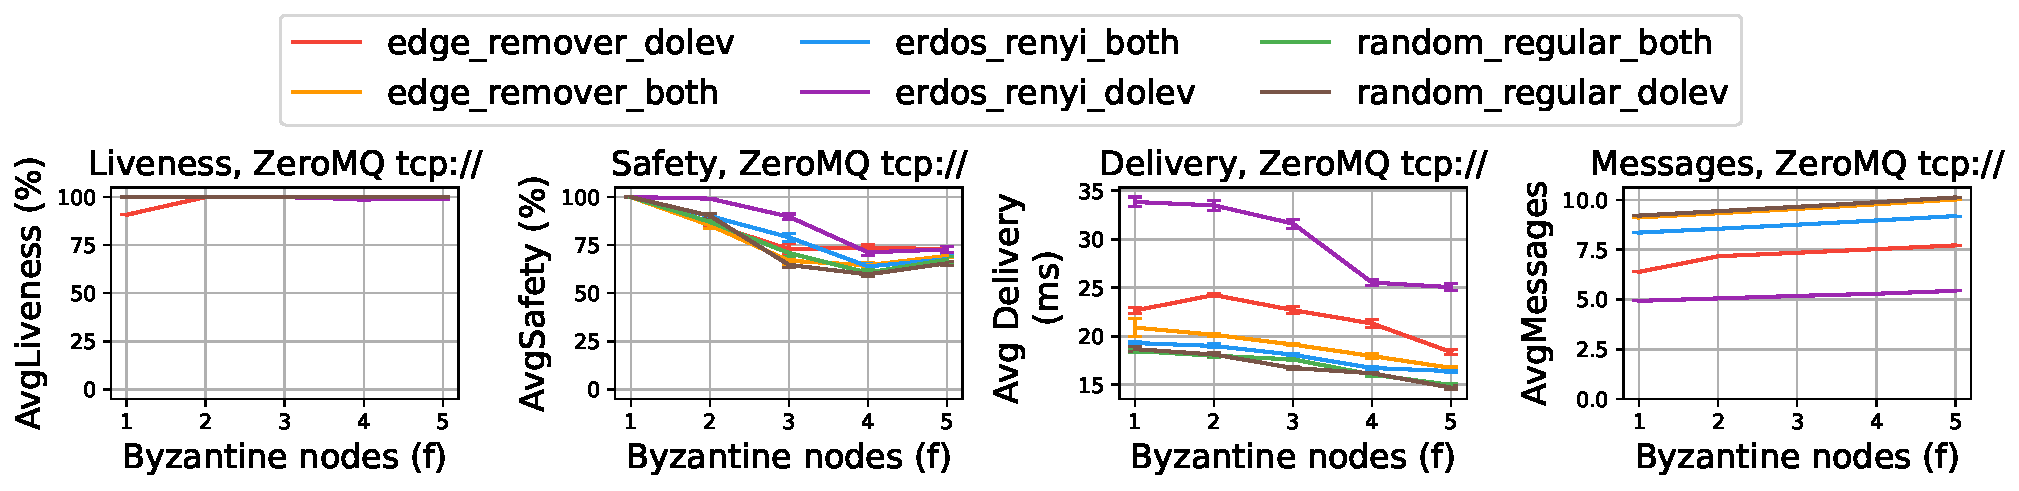
\includegraphics[width=\textwidth]{../figures/n50_tcp.pdf}
  \caption{The experiments of Figure~\ref{fig:one-node} on ZeroMQ over \code{tcp://}, across
    11 cluster nodes. Same metrics, aggregation and confidence intervals.}
  \label{fig:tcp}
\end{figure}

Moving the peers across machines leaves liveness and messages unchanged: liveness averages 99.6\%
and a correct peer sends 8.35 messages, as on one node. Delivery is slower, 17.7 to 22.3\,ms against
16.7 to 19.6\,ms over \code{ipc://}. Safety is lower once $f$ exceeds $t_s$: at $f = 4$ it averages
65.6\%, against 73.0\% over \code{ipc://} and 77.4\% on Abstract.

\subsection{Execution time}

Table~\ref{tab:time} gives the time one run of the 300 experiments takes on each backend, measured
from the launch of each experiment until all its processes have exited. Between runs it ranges from
138 to 153\,s on Abstract, 258 to 263\,s on BoostMq, 138 to 144\,s on ZeroMQ over \code{ipc://} and
1,245 to 1,252\,s over \code{tcp://}.

\begin{table}[!htbp]
  \centering
  \begin{tabular}{llrr}
    \toprule
    Backend & Deployment & Time per run (s) & Per experiment (s) \\
    \midrule
    Abstract & one node & 149 & 0.50 \\
    BoostMq & one node & 260 & 0.87 \\
    ZeroMQ \code{ipc://} & one node & 141 & 0.47 \\
    ZeroMQ \code{tcp://} & 11 nodes & 1,249 & 4.16 \\
    \bottomrule
  \end{tabular}
  \caption{Mean execution time over the 10 runs. Builds are not included.}
  \label{tab:time}
\end{table}

On one node, ZeroMQ is as fast as Abstract. On 11 nodes, this time also includes starting and
stopping the peers on the 10 remote nodes over \code{oarsh} for every experiment.

\bibliographystyle{plain}
\bibliography{references}

\end{document}
